\section{Factorial analysis on different number of nodes}
The purpose of this section is to confront the results of the factorial analysis for various models with different number of nodes, since the process for obtaining these results is the same explained in section \ref{sec:ModelFitting}, we shall skip directly to the values for influences.
\subsection{Influence on coverage rate and time}
We first analyze the result for the coverage percentage and the coverage time.

\begin{table}[H]\label{tab:CovPerc}
\centering
\begin{tabular}{|c|c|c|c|}
\hline
\textbf{Number of   nodes} & \textbf{Probability} & \textbf{Radius} & \textbf{Combined} \\ \hline
\textbf{50} & \textit{0,0021} & 0,9961 & \textit{0,0018} \\ \hline
\textbf{100} & \textit{0,0054} & 0,9939 & \textit{0,0007} \\ \hline
\textbf{200} & \textit{0,4036} & 0,4476 & 0,1488 \\ \hline
\textbf{500} & \textit{0,9048} & \textit{0,0464} & \textit{0,0488} \\ \hline
\textbf{700} & \textit{0,9580} & \textit{0,0208} & \textit{0,0212} \\ \hline
\end{tabular}
\caption{Influences for coverage percentage}
\end{table}

\begin{table}[H]\label{tab:CovTime}
\centering
\begin{tabular}{|c|c|c|c|}
\hline
\textbf{Number of   nodes} & \textbf{Probability} & \textbf{Radius} & \textbf{Combined} \\ \hline
\textbf{50} & \textit{0,8269} & 0,1148 & \textit{0,0584} \\ \hline
\textbf{100} & \textit{0,9819} & \textit{0,0108} & \textit{0,0073} \\ \hline
\textbf{200} & \textit{0,6672} & \textit{0,2372} & 0,0956 \\ \hline
\textbf{500} & \textit{0,9571} & \textit{0,0336} & \textit{0,0092} \\ \hline
\textbf{700} & \textit{0,9646} & \textit{0,0060} & \textit{0,0294} \\ \hline
\end{tabular}
\caption{Influences for coverage time}
\end{table}


To draw easier conclusion, in the following section, these result are plotted in a scatter plot with lines. Note that the values in italic are referred to influence of factors with a negative contribution meaning that a higher value for that specific factor produce a lower output, however this is not a bad thing because in the case of the coverage time the objective is to reduce it, not increase it.

\begin{figure}[H]\label{pic:CovPerc}
\centering
    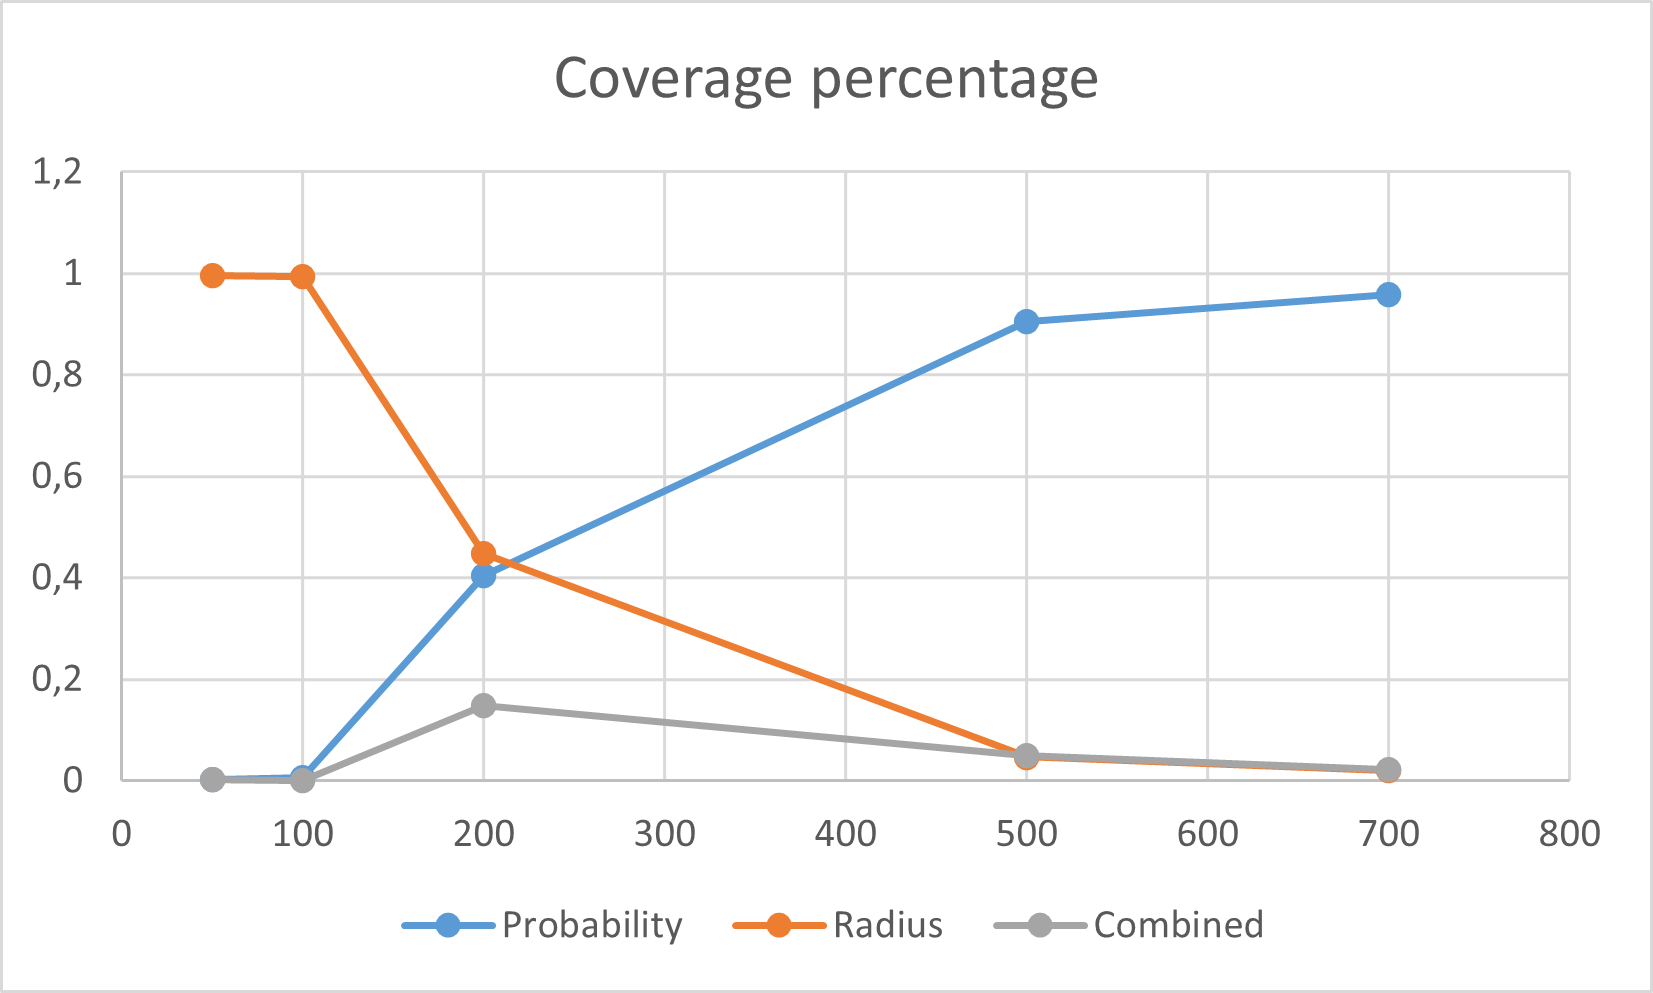
\includegraphics[width= 1\textwidth]{./images/CoveragePercentageWithNodes.png}
    \caption{Coverage percentage at different nodes}
    \label{fig:immagine}
\end{figure}


\begin{figure}[H]
\centering
    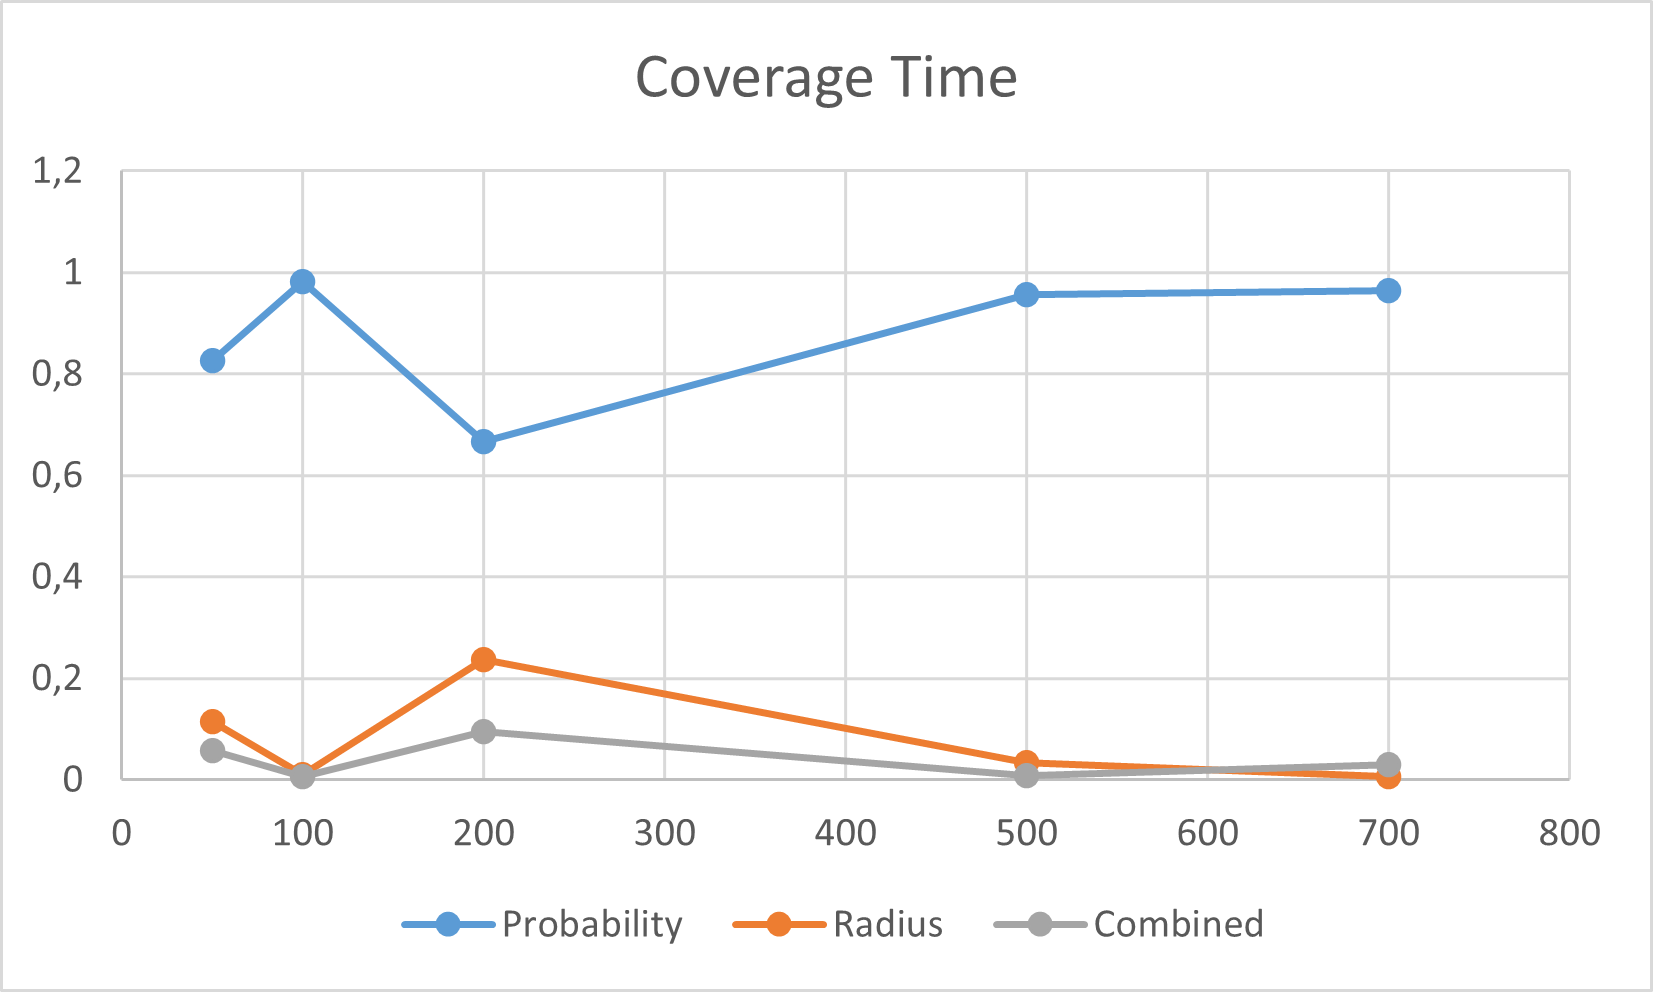
\includegraphics[width= 1\textwidth]{./images/CoverageTimeWithNodes.png}
    \caption{Coverage time at different nodes}
    \label{fig:immagine}
\end{figure}

Let's start with Figure \ref{pic:CovPerc} it is easy to understand that a low density the radius is far more critical then the probability since with low radius it is likely that many nodes are isolated or do not get a second "chance" after receiving a collision. At high number of nodes, the contrary happens the reason of this behavior is that even with low radius each node as a lot of neighbors so it is far more important for them to avoid collision, this is achieved by a low probability as seen in the boxplot and as indicated in section \ref{subsec:CovPerc}.

The coverage time is more tricky to understand, with a high number of nodes it is far more important for the nodes to quickly transmit. However with a low density the behavior for the influences is more chaotic, this happens because, since this analysis takes account only for the coverage time, some runs end immediately with a high probability and low radius however these configurations result in a very low coverage percentage. With 200 nodes a critical point is reached, the reason behind is that this configuration has a high enough density for the runs to not immediately terminate as in the previous cases. This still determines a high influence for the probability factor, but still gains from a higher radius so that more nodes are reached at each transmission. Note that almost all of the values for influence in table \ref{tab:CovTime} are in italics, this make sense because our objective is to diminish the coverage time overall.

\subsection{Analysis on the models parameters}
The next step is to perform the same confrontation for the models parameters, obviously the Gompertz model is used since it was already concluded to be the most fitting one

\begin{table}[H]
\centering
\begin{tabular}{|c|c|c|c|}
\hline
\textbf{Number of   nodes} & \textbf{Probability} & \textbf{Radius} & \textbf{Combined} \\ \hline
\textbf{50} & \textit{0,0020} & 0,9962 & \textit{0,0018} \\ \hline
\textbf{100} & \textit{0,0054} & 0,9939 & \textit{0,0007} \\ \hline
\textbf{200} & \textit{0,4095} & 0,4366 & 0,1539 \\ \hline
\textbf{500} & \textit{0,8990} & \textit{0,0578} & \textit{0,0431} \\ \hline
\textbf{700} & \textit{0,9514} & \textit{0,0317} & \textit{0,0169} \\ \hline
\end{tabular}
\caption{Influence for the asymptote}
\end{table}

\begin{table}[H]
\centering
\begin{tabular}{|c|c|c|c|}
\hline
\textbf{Number of   nodes} & \textbf{Probability} & \textbf{Radius} & \textbf{Combined} \\ \hline
\textbf{50} & \textit{0,2325} & 0,0580 & \textit{0,7096} \\ \hline
\textbf{100} & \textit{0,5492} & \textit{0,3096} & \textit{0,1412} \\ \hline
\textbf{200} & \textit{0,0666} & \textit{0,9010} & \textit{0,0324} \\ \hline
\textbf{500} & \textit{0,0025} & \textit{0,9851} & \textit{0,0124} \\ \hline
\textbf{700} & \textit{0,0016} & \textit{0,9902} & \textit{0,0082} \\ \hline
\end{tabular}
\caption{Influence for the displacement}
\end{table}




\begin{table}[H]\label{tab:Growth}
\centering
\begin{tabular}{|c|c|c|c|}
\hline
\textbf{Number of   nodes} & \textbf{Probability} & \textbf{Radius} & \textbf{Combined} \\ \hline
\textbf{50} & 0,9444 & 0,0021 & \textit{0,0535} \\ \hline
\textbf{100} & 0,3672 & 0,3468 & 0,2860 \\ \hline
\textbf{200} & 0,5578 & 0,3791 & 0,0631 \\ \hline
\textbf{500} & 0,9044 & 0,0280 & 0,0676 \\ \hline
\textbf{700} & 0,9586 & \textit{0,0110} & 0,0304 \\ \hline
\end{tabular}
\caption{Influence for the growth rate}
\end{table}

As previously done, the same kind of scatter plot is shown underneath to better understand the patterns, the values in italic have the same meaning as in the previous section.

\begin{figure}[H]\label{pic:AsymptoteNodes}
\centering
    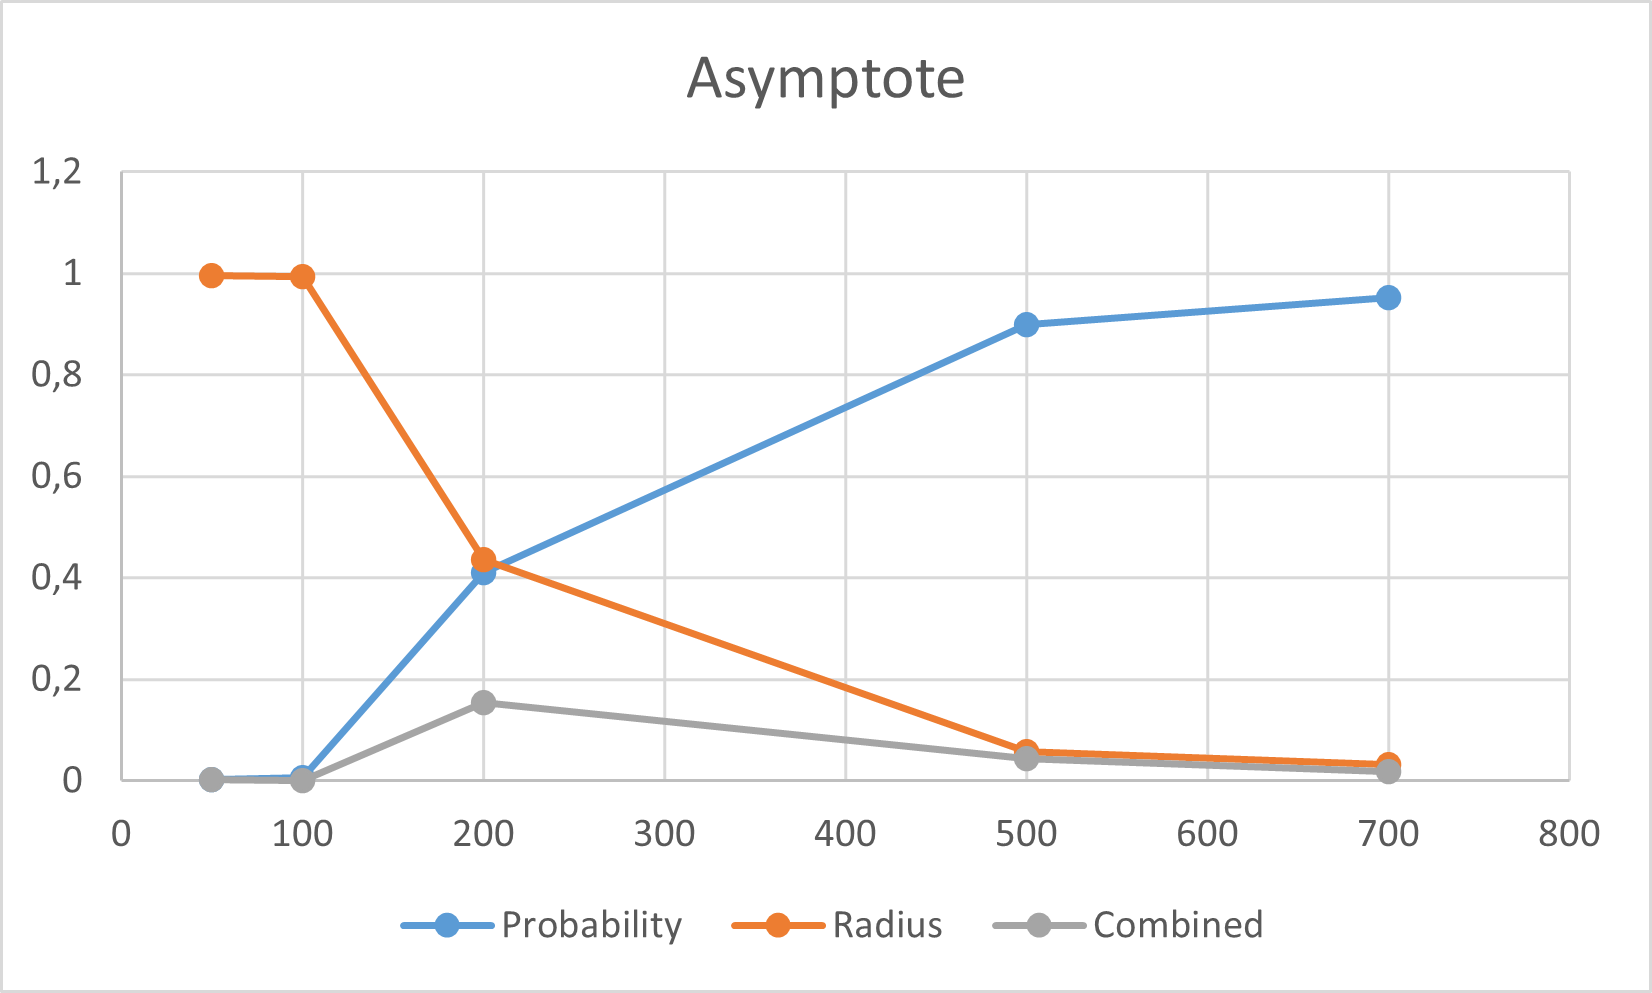
\includegraphics[width= 1\textwidth]{./images/AsymptoteWithNodes.png}
    \caption{Asymptote influences at different nodes}

\end{figure}

As expected the influences for the asymptote are similar to the one for the coverage percentage, so it is unnecessary to repeat the same explanation.

\begin{figure}[H]\label{pic:DisplacementNodes}
\centering
    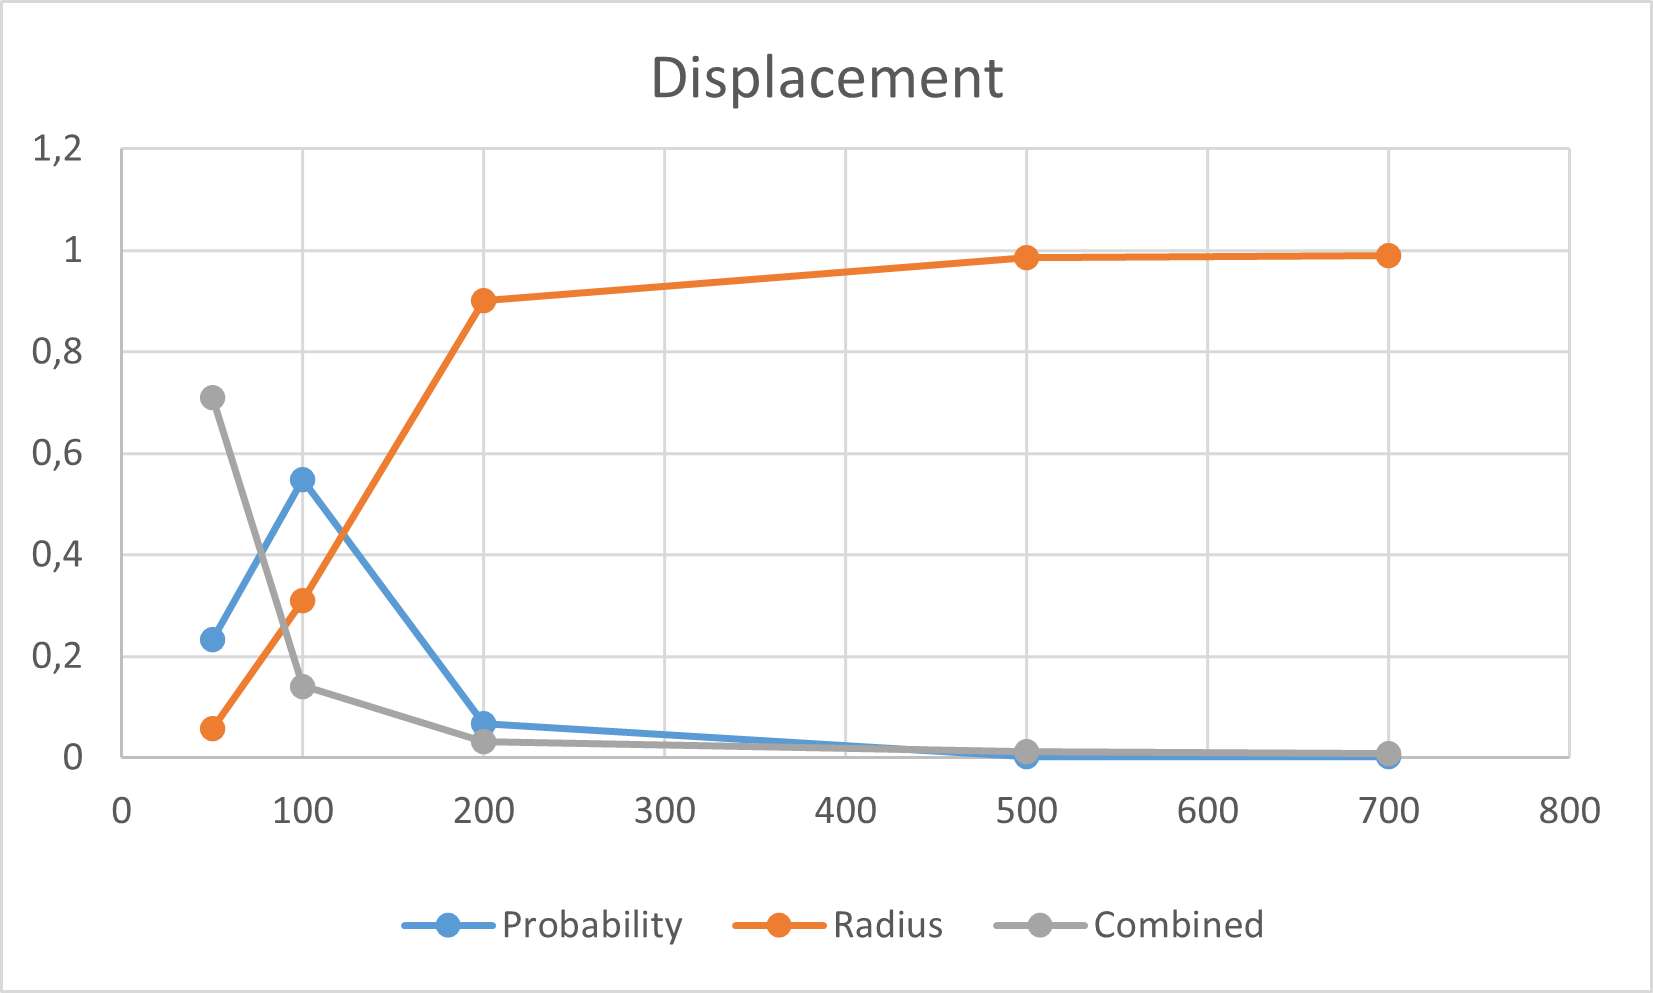
\includegraphics[width= 1\textwidth]{./images/DisplacementWithNodes.png}
    \caption{Displacement influences at different nodes}
\end{figure}

At low density to achieve a high displacement it is necessary to have a high combined effort so that the many neighbors of patient zero node can transmit immediately. With a growing density the radius influence takes up with a "quantity over quality" logic where, even with low probability, a high radius allow the first infected node to reach a great number of nodes, generating a lower displacement (the influence are referencing factors with negative influence) even if some nodes do not immediately re-transmit.

\begin{figure}[H]\label{pic:GrowthRatesNodes}
\centering
    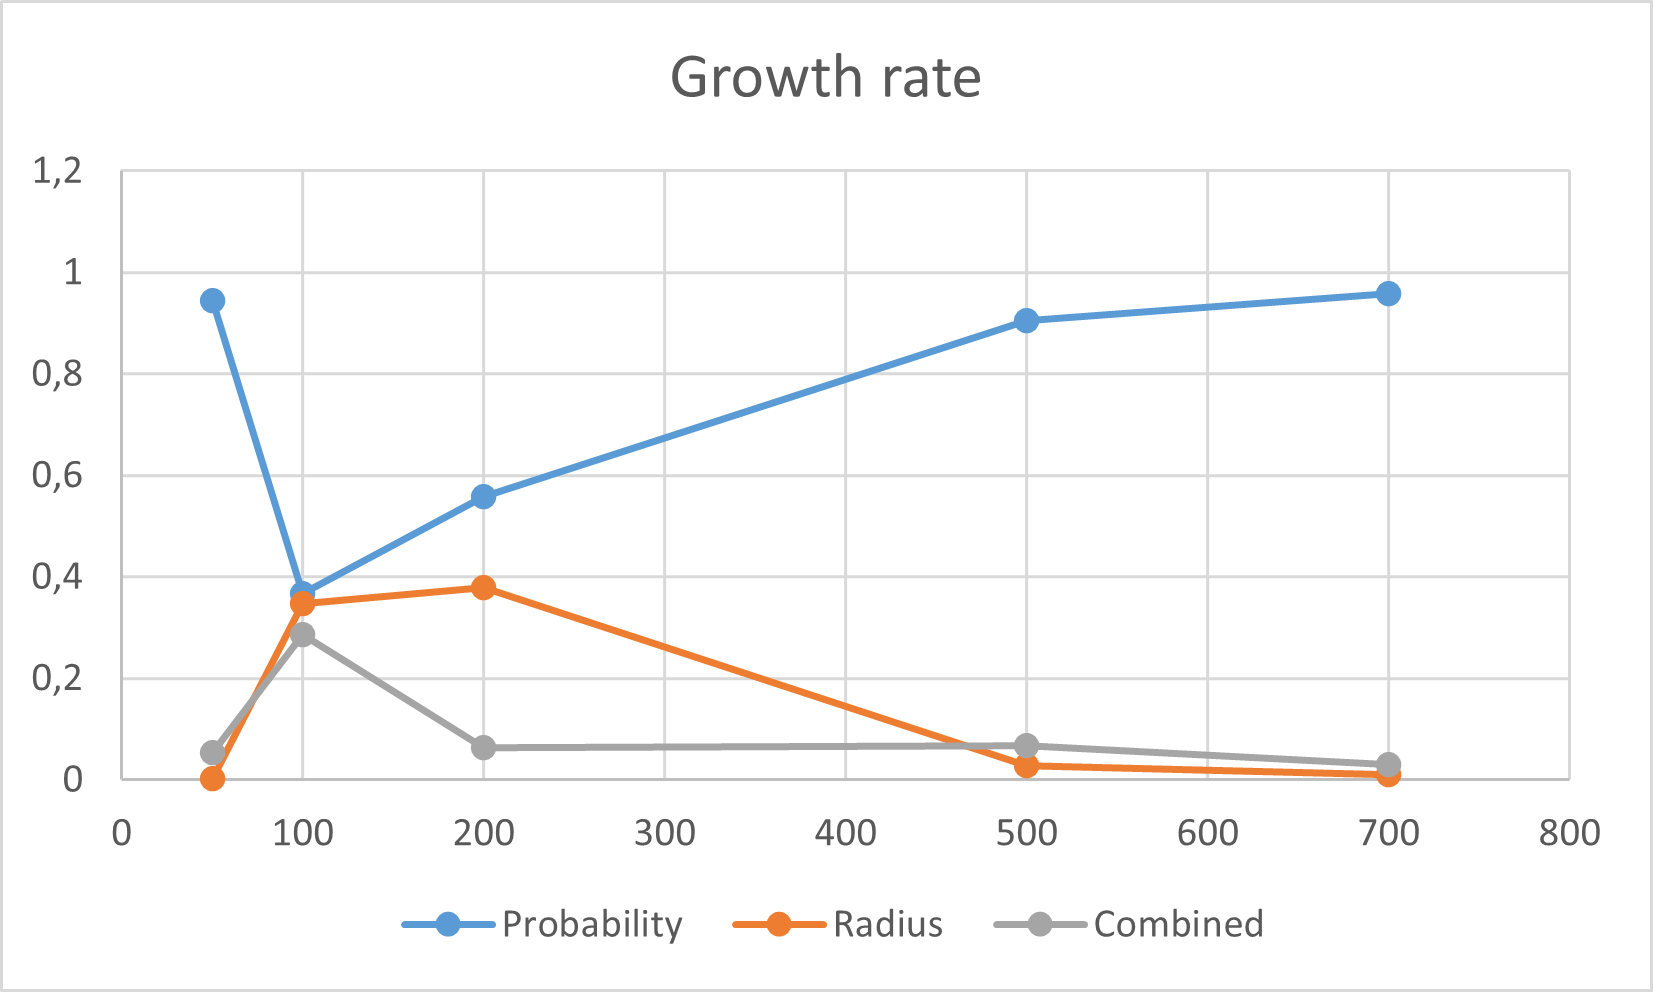
\includegraphics[width= 1\textwidth]{./images/GrowthRateWithNodes.png}
    \caption{Growth rate influences at different nodes}
\end{figure}

For the growth rate it is easy to understand that at high density the probability is the most influencing factor since, even with low radius, nodes tend to have many neighbors. With low density the results are similar, but for another reason. In these conditions, nodes have few neighbors so it is imperative for them to immediately re-transmit the infection message. It is also important to notice that even with a high radius, nodes would not have many more neighbors. At medium density the influence of the factors tends to be more equally distributed; this makes sense because a high probability is still helpful as previously said and a high radius allows the node to have many more neighbors.

